\documentclass[UTF8]{ctexart}
\usepackage{fullpage}
\usepackage{times}
\usepackage[normalem]{ulem}
\usepackage{multirow}
\usepackage{fancyhdr,graphicx,amsmath,amssymb, mathtools, scrextend, titlesec, enumitem}\usepackage[pdftex]{hyperref}
\usepackage[ruled,vlined]{algorithm2e}
\usepackage{parskip}
\usepackage{listings}
\usepackage{amsmath}
\usepackage{physics}
\usepackage{bbm}
\usepackage{titling}
\usepackage{bm}
\usepackage{geometry}
\geometry{top=1cm, left=1cm, bottom=1.5cm, right=1.5cm, margin=1cm}
\newcommand{\varvec}[2][n]{#2_1,\ldots, #2_#1}
\newcommand{\Var}{\mathrm{Var}}
\newcommand{\Bias}{\mathrm{Bias}}
\newcommand{\Cov}{\mathrm{Cov}}
\newcommand{\E}{{\rm I\kern-.3em E}}
\newcommand{\Binomial}{\mathrm{Binomial}}
\newcommand{\Bernoulli}{\mathrm{Bernoulli}}
\newcommand{\Poisson}{\mathrm{Poisson}}
\newcommand{\Normal}{\mathcal{N}}
\newcommand{\one}{\mathbbm{1}}
\newcommand{\Beta}{\text{Beta}}
\newcommand{\BetaPDF}{\text{Beta}}
\newcommand{\GammaPDF}{\text{Gamma}}
\newcommand{\Uniform}{\mathrm{Uniform}}
\newcommand{\QED}{\newline \mbox{} \hfill $\blacksquare$}
\newcommand{\Real}{\mathbb{R}}
\newcommand{\Sgn}{\mbox{Sgn}}
\renewcommand*{\arraystretch}{1.4}
\newtheorem{theorem}{Result}
\newtheorem{definition}{Definition}
\lstset{frame=tb,
	language=Python,
	aboveskip=3mm,
	belowskip=3mm,
	showstringspaces=false,
	columns=flexible,
	basicstyle={\small\ttfamily},
	numbers=none,
	stringstyle=\color{mauve},
	breaklines=true,
	breakatwhitespace=true,
	tabsize=3
}
\graphicspath{ {./imgs} }

\title{Image Processing}
\begin{document}
	\maketitle
	
\section{Image}
\begin{definition}
	\textbf{Radiance} is the total amount of energy that flows from the light source, measured in watts(W). 
\end{definition}

\begin{definition}
	\textbf{Luminance}, measured in lumens(lm), gives a measure of the amount of energy an observer perceives from a light source
\end{definition}
	
\begin{definition}
	An  \textbf{image} is a function  $l = f(x, y)$ of real valued plane coordinates where $l$ is called \textbf{intensity} or \textbf{gray level}. If all values are finite and discrete, it is called a \textbf{digital image}. And 
	$$ l =  f(x, y) = i(x, y) r(x, y), \quad l \in [L_{\min}, L_{\max}]$$
	where $i(x, y) \in [0, \infty)$ is called \textbf{illumination}, $r(x, y)\in [0, 1]$ is called \textbf{reflectance}.  $L_{\min} = i_{\min}r_{\min}$ and $L_{\max} = i_{\max}r_{\max}$. The interval $[L_{\min}, L_{\max}]$ is called \textbf{intensity(gray) scale}
\end{definition}

Illumination Example: On a clear day, the sun may produce in excess of $90,000$ lm/m$^2$ of illumination on the surface of earth; less than $10,000$ lm/m$^2$ on a cloudy day. On a clear evening, a full moon is about $0.1$ lm/m$^2$. Typical illumination level in a commercial office is about $1,000$ lm/m$^2$.

Reflectance Example ($r(x, y)$): 0.01 for black velvet, 0.65 for stainless steel, 0.8 for flat-white wall paint, 0.93 for snow, 0.9 for silver-plated metal.

Gray scale Example: $L_{\min} \approx 10$ and $L_{\max} \approx 1000$ are typical indoor values in absence of additional illumination. Common practice shifts the gray scale interval to $[0, 1]$

\section{Digitizing an image}
\begin{definition}
	Let $f(s, t)$ be a continuous image. Digitizing the coordinate values is called \textbf{sampling}. Digitizing the amplitude(intensity) values is called \textbf{quantization}. In digital sotrage and quantizing hardware, the number of intensity levels $L$ is usually an integer power of 2, $L=2^k$ . The discrete levels $[0, L-1]$ are equally spaced.
\end{definition}

\begin{center}
	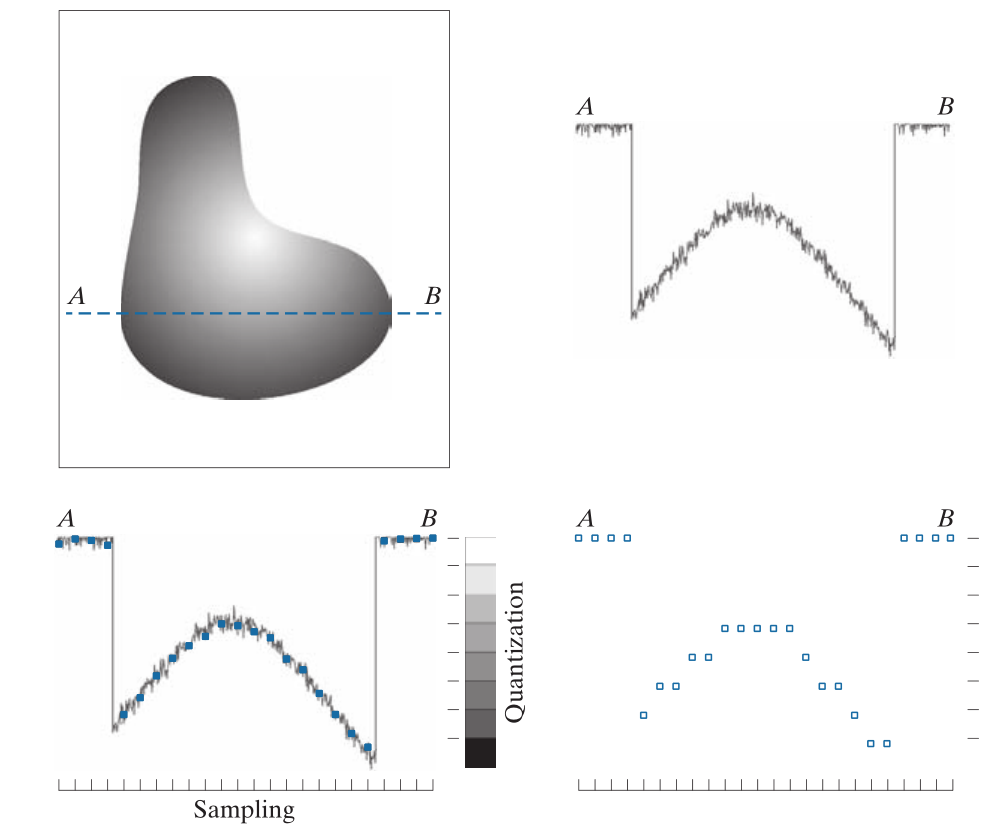
\includegraphics[scale=0.5]{digitization.png}
\end{center}

\begin{definition}
	The \textbf{dynamic range(动态范围)} of an imaging system is the ratio of max measurable intensity to the minimum detectable intensity level in the system. Note that this is used to describe imaging system NOT an image. 
	\textbf{image contrast} is used to describe an image's highest and lowest intensity difference.
\end{definition}
As a rule, the upper limit is determined by \textbf{saturation} and the lower limit by \textbf{noise}.

\begin{center}
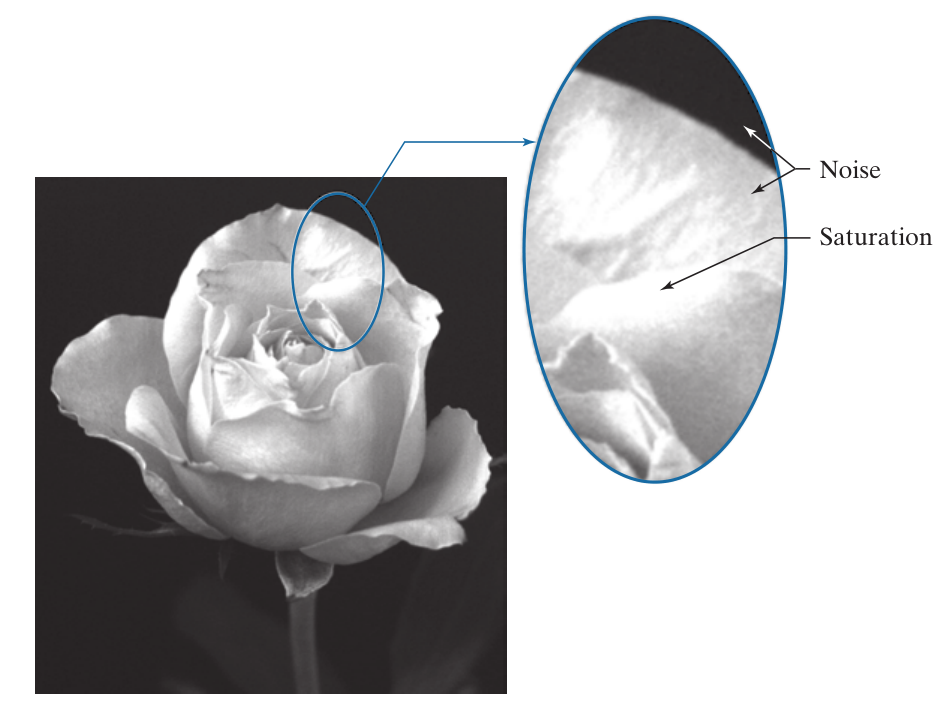
\includegraphics[scale=0.5]{dynamic_range.png}
\end{center}

Example: An image can have $2^k$ possible intensity levels referred to as "k-bit" image. An image with 256 gray levels is called an 8-bit image. The space needed to store a 8-bit image is $N \times M \times 1 \text{byte}$.

\subsection{Spatial and intensity resolution}
\begin{definition}
	\textbf{Spatial resolution} is a measure of the smallest discernible details in an image. It can be measured in 
	\begin{itemize}
		\item \textit{line pairs per unit distance}: alternating black and white lines each with width $W$.
		\item \textit{largest number of discernible lines pairs per unit distance}
		\item \textit{dots(pixels) per unit distance}. For example, dpi(dot per inch) in US.
	\end{itemize}
\end{definition}

Example: Newspaper printed with resolution of 75dpi, magazines at 133dpi, brochures at 175dpi, textbook page at 2400dpi.

\begin{definition}
	\textbf{Intensity resolution} refers to the smallest discernible change in intensity level. Since intensity level is quantized as an integer power of 2. It is common practice to refer to the number of bits used to quantize intensity as the intensity resolution. 
\end{definition}

Example: an image's intensity quantized as 256 levels uses 8 bit so the intensity resolution is 8 bit.

\end{document}